\documentclass[12pt]{article}
\usepackage{geometry}                % See geometry.pdf to learn the layout options. There are lots.
\geometry{letterpaper}                   % ... or a4paper or a5paper or ... 
%\geometry{landscape}                % Activate for for rotated page geometry
\usepackage[parfill]{parskip}    % Activate to begin paragraphs with an empty line rather than an indent
\usepackage{daves,fancyhdr,natbib,graphicx,dcolumn,amsmath,lastpage,url}
\usepackage{amsmath,amssymb,epstopdf,longtable}
\usepackage{paralist}  % need to properly formulate standard answer blocks
\usepackage[final]{pdfpages}
\DeclareGraphicsRule{.tif}{png}{.png}{`convert #1 `dirname #1`/`basename #1 .tif`.png}
\pagestyle{fancy}
\lhead{CE 3305 Fluid Mechanics; Final Exam Part 2 (In Class)}
\rhead{Name:\_\_\_\_\_\_\_\_\_\_\_\_\_\_\_\_\_\_\_\_\_\_\_\_\_\_\_\_\_\_\_\_\_\_}
\lfoot{REVISION A}
\cfoot{}
\rfoot{Page \thepage\ of \pageref{LastPage}}
\renewcommand\headrulewidth{0pt}
%%%%%%%%%%%%%%%%%%%%%%%%%%%%%%%%%%%%
\begin{document}
%%%%%%%%%%%%%%%%%%%%%%%%%%%%%%%%%%%
\begingroup
\begin{center}
{\textbf{{ CE 3305 Engineering Fluid Mechanics} \\ Final Exam (Part 2) \\ Summer 2019 -- GERMANY} }
\end{center}
\endgroup
\begingroup
~\newline

\begin{enumerate}
%\item (Problem 9.42 pg 355) A flat plate 1.5 $m$ long and 1.0 $m$ wide is towed in water at 20$^oC$ in the direction of its length and at a speed of 15 $cm/s$.  Determine the resistance of the plate and the boundary layer thickness at its aft end.
%
%\item (Problem 9.48 pg 355) An airplane wing of 2$m$ chord length (leading edge to trailing edge distance)and 11 $m$ span flies at 200 $km/hr$ in air at 30$^oC$.  Assume the resistance of the wing surfaces is like that of a flat plate.
%\begin{enumerate}
%\item What is the friction drag on the wing?
%\item What power will be required to overcome this friction?
%\item How much of the chord is laminar?
%\item What will be the change in drag if a turbulent boundary layer is tripped at the leading edge?
%\end{enumerate}


\item Figure \ref{fig:WindDrum} is a schematic of wind blowing on a petroleum storage drum.  Estimate the wind speed (in meters per second) needed to tip the drum over.  \\~\\ The mass of the drum is 25 kilograms, the diameter is 55 centimeters, and the height is 90 centimeters.  \\~\\The density of air is $\rho = 1.23~kg/m^3$  \\ The viscosity of air is $\nu = 1.46 \times 10^{-5}~m^2/s$
\begin{figure}[htbp] %  figure placement: here, top, bottom, or page
   \centering
   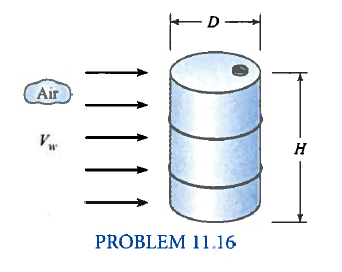
\includegraphics[width=2in]{WindDrum.jpg} 
   \caption{Wind blowing over a storage drum}
   \label{fig:WindDrum}
\end{figure}


\end{enumerate}
\end{document}  